\documentclass[polish,a4paper]{article}
\usepackage{amsmath}
\usepackage{amssymb, amsfonts, amsthm, amsmath, bm}
\usepackage[T1]{fontenc}
\usepackage[utf8]{inputenc}
\usepackage{babel}
\usepackage{pslatex}
\usepackage{pgfplots}
\usepackage{hhline}
\usepackage[american]{circuitikz} 
\usepackage{anysize}
\usepackage{graphicx}
\DeclareGraphicsExtensions{.jpg}
\marginsize{2.5cm}{2.5cm}{3cm}{3cm}
\bibliographystyle{IEEEtran}


%makro do indeksów w tabeli
\newcommand{\PRzFieldDsc}[1]{\sffamily\bfseries\scriptsize #1}

%makro do informacji w tabeli
\newcommand{\PRzFieldCnt}[1]{\itshape #1}

%potężne makro tworzące tabelę z informacjami o teamie
\newcommand{\PRzHeading}[8]{
%% #1 - nazwa laboratorium
%% #2 - kierunek 
%% #3 - specjalność 
%% #4 - rok studiów 
%% #5 - symbol grupy lab.
%% #6 - temat 
%% #7 - numer lab.
%% #8 - skład grupy ćwiczeniowej

\begin{center}
\begin{tabular}{ p{0.32\textwidth} p{0.15\textwidth} p{0.15\textwidth} p{0.12\textwidth} p{0.12\textwidth} }

  &   &   &   &   \\
\hline
\multicolumn{5}{|c|}{}\\[-1ex]
\multicolumn{5}{|c|}{{\LARGE #1}}\\
\multicolumn{5}{|c|}{}\\[-1ex]

\hline
\multicolumn{1}{|l|}{\PRzFieldDsc{Kierunek}}	& \multicolumn{1}{|l|}{\PRzFieldDsc{Specjalność}}	& \multicolumn{1}{|l|}{\PRzFieldDsc{Rok studiów}}	& \multicolumn{2}{|l|}{\PRzFieldDsc{Symbol grupy lab.}} \\
\multicolumn{1}{|c|}{\PRzFieldCnt{#2}}		& \multicolumn{1}{|c|}{\PRzFieldCnt{#3}}		& \multicolumn{1}{|c|}{\PRzFieldCnt{#4}}		& \multicolumn{2}{|c|}{\PRzFieldCnt{#5}} \\

\hline
\multicolumn{4}{|l|}{\PRzFieldDsc{Temat Laboratorium}}		& \multicolumn{1}{|l|}{\PRzFieldDsc{Numer lab.}} \\
\multicolumn{4}{|c|}{\PRzFieldCnt{#6}}				& \multicolumn{1}{|c|}{\PRzFieldCnt{#7}} \\

\hline
\multicolumn{5}{|l|}{\PRzFieldDsc{Skład grupy ćwiczeniowej oraz numery indeksów}}\\
\multicolumn{5}{|c|}{\PRzFieldCnt{#8}}\\

\hline
\multicolumn{3}{|l|}{\PRzFieldDsc{Uwagi}}	& \multicolumn{2}{|l|}{\PRzFieldDsc{Ocena}} \\
\multicolumn{3}{|c|}{\PRzFieldCnt{\ }}		& \multicolumn{2}{|c|}{\PRzFieldCnt{\ }} \\

\hline
\end{tabular}
\end{center}
}
%koniec potężnego makro do tabeli

\begin{document}

%stworzenie tabeli - miejsce na zmienianie danych w tabeli
%indeksy do uzupełnienia
\PRzHeading{Laboratorium Podstaw Elektroniki}{Informatyka}{--}{I}{I1}{Rezonans w obwodach RLC}{3}{Ewa Fengler(132219), Sebastian Maciejewski(132275), Jan Techner(132332)}{}

%ZADANIA

\section*{Cel}
Celem przeprowadzanego doświadczenia jest zapoznanie się ze zjawiskiem rezonansu szeregowego w obwodzie RLC.
W tym celu wykonywane są kolejno zadania:

\section{Zadanie 1.}
Rozpatrywany obwód wraz z wybranymi wartościami elementów. \\
Wyznaczona przez prowadzącego wartość pojemności kondensatora użytego w doświadczeniu to 13.3nF. \\

\begin{figure}[!h]
\centering
\begin{circuitikz}[scale=1.1, font = \scriptsize]
\draw (-0.3,1) to [sinusoidal voltage source, l^=$V_{pp}$, a_=$8V$, o-o] (-0.3,-1)
	  (-0.3,1) -- (1,1)
	  (-0.3,-1) -- (1,-1)
	  (2,1) to [short, -*] (2.5,1) -- (2.5, 2.5) to [voltmeter, -*] (4, 2.5) to [voltmeter] (5.5, 2.5) to [short, -*] (5.5, 1) to [short, -*] (6,1) to [R, l=$R_1$, a=1k$\Omega$, *-*] (6,-1) -- (2,-1) 
	  (4,2.5) to [short, -*] (4,1) 
	  (2.5,1) to [C, l=$C_1$, a=13.3nF] (4,1) to [L, l=$L_1$, a=66mH] (5.5,1)
	  (6,1) -- (7.5,1) 
	  (6,-1) -- (7.5,-1)
	  (1.5,-2.3) to [short, -o] (3, -2.3)
	  (1.5,-3) to [short, -o] (3, -3)
	  (5,-2.3) to [short, -o] (6.5, -2.3)
	  (5,-3) to [short, -o] (6.5, -3);
\draw [line width = 2, blue] (1,1) -- (1,-1) -- (2,-1) -- (2, 1)
	  (1.5, -1) -- (1.5, -3)
	  (7.5,1) -- (7.5,-1.7) -- (5,-1.7) --(5,-3)  ;  
\draw [line width = 1, dashed, gray] (2.2,1.9) -- (6.7,1.9) -- (6.7,-1.2) -- (2.2, -1.2) -- (2.2,1.9); 
\draw (0.5,1.1) node {czerw.}
	  (0.5,-0.9) node {biały}
	  (7.2,1.1) node {czerw.}
	  (7.2,-0.9) node {biały}
	  
	  (2.6, -2.2) node {czerw.}
	  (2.6, -2.9) node {biały}
	  (6.1, -2.2) node {czerw.}
	  (6.1, -2.9) node {biały}
	  (1.5, -0.8) node {BNC}
	  (5.5,-1.5) node {BNC}
      (1.3, -2) node[rotate=90] {BNC}
      (3.3, -2.65) node[rotate=90] {\small\textbf{kanał X}}
      (6.8, -2.65) node[rotate=90] {\small\textbf{kanał Y}}
      (-1.1, 0.4) node {sinus}
      (-1.45, -0.4) node {f = 1...15kHz} 
	  ;
\end{circuitikz}
\caption{Badany obwód}
\label{fig:badobw}
\end{figure}
$\newline$
Wartości elementów obwodu : $V_{pp} = 4V$, $R_1 = $1k$\Omega$,  $C_1 = 13.3$nF,  $L_1 = 66$mH
\newpage

\section{Zadanie 2.}

Wartości elementów użytych do zbudowania obwodu przedstawionego na rysunku \ref{fig:badobw}.

\begin{center}
\begin{tabular}{|c||c|c|c|c|}
\hline
\textbf{Element} & \textbf{Wartość zadana} & \textbf{Oznaczenie} & \textbf{Wartość odczytana} & \textbf{Wartość zmierzona}\\
\hhline{|=#=|=|=|=|}
\textbf{Rezystor} & $1k\Omega$ & brązowy, czarny, czerwony, złoty & $1000\Omega\pm5\%$ & $976,6\Omega\pm5\%$\\
\hline
\textbf{Cewka} & $66mH$ & --- & --- & $69,78mH$ (Opór: $123,3\Omega$)\\
\hline
\textbf{Kondensator} & $13,3nF$ & 332 (4 szt.) & $3,3nF$ x 4  & $13,25nF$\\
\hline
\end{tabular}
\end{center}


\section{Zadanie 5.}
Wyniki pomiarów napięć na rezystancji, pojemności i  indukcyjności oraz napięcia na źródle w zależności od częstotliwości pobudzenia przedstawione w tabeli.
\begin{center}
\begin{tabular}{|c|c|c|c|c|c|}
\hline
\textbf{Lp.} & \textbf{Częstotliwość} & \textbf{$V_{rms}(1)$ źródło} & \textbf{$V_{rms}(2)$ rezystor} & \textbf{Napięcie na kondensatorze} & \textbf{Napięcie na cewce}\\
\hline
1. & $2,26kHz$ & $1,33V$ & $0,31V$ & $1,6V$ & $0,34V$\\
\hline
2. & $2,83kHz$ & $1,34V$ & $0,43V$ & $1,81V$ & $0,59V$\\
\hline
3. & $3,34kHz$ & $1,33V$ & $0,59V$ & $2,07V$ & $0,95V$ \\
\hline
4. & $3,83kHz$ & $1,31V$ & $0,77V$ & $2,37V$ & $1,44V$\\
\hline
5. & $4,36kHz$ & $1,30V$ & $1,00V$ & $2,65V$ & $2,17V$\\
\hline
6. & $4,85kHz$ & $1,39V$ & $1,21V$ & $2,82V$ & $2,85V$\\
\hline
7. & $5,00kHz$ & $1,37V$ & $1,18V$ & $2,68V$ & $2,87V$\\ 
\hline
8. & $5,15kHz$ & $1,35V$ & $1,17V$ & $2,59V$ & $3,00V$\\
\hline
9. & $5,23kHz$ & $1,35V$ & $1,11V$ & $2,59V$ & $2,98V$\\
\hline
10. & $5,34kHz$ & $1,35V$ & $1,08V$ & $2,38V$ & $2,96V$\\
\hline
11. & $5,39kHz$ & $1,35V$ & $1,10V$ & $2,33V$ & $2,99V$\\
\hline
12. & $5,42kHz$ & $1,35V$ & $1,11V$ & $2,33V$ & $2,99V$\\
\hline
13. & $5,56kHz$ & $1,37V$ & $1,06V$ & $2,17V$ & $2,93V$\\
\hline
14. & $5,96kHz$ & $1,37V$ & $0,91V$ & $1,80V$ & $2,80V$\\
\hline
15. & $6,99kHz$ & $1,39V$ & $0,67V$ & $1,12V$ & $2,38V$\\
\hline
16. & $7,82kHz$ & $1,40V$ & $0,55V$ & $0,80V$ & $2,14V$\\
\hline
17. & $8,63kHz$ & $1,41V$ & $0,46V$ & $0,60V$ & $2,00V$\\
\hline
18. & $9,61kHz$ & $1,43V$ & $0,40V$ & $0,45V$ & $1,86V$\\
\hline
19. & $10,88kHz$ & $1,38V$ & $0,33V$ & $0,31V$ & $1,70V$\\
\hline
20. & $11,60kHz$ & $1,39V$ & $0,30V$ & $0,26V$ & $1,65V$\\
\hline
21. & $12,67kHz$ & $1,38V$ & $0,26V$ & $0,21V$ & $1,60V$\\
\hline
22. & $15,00kHz$ & $1,39V$ & $0,22V$ & $0,13V$ & $1,54V$\\
\hline
\end{tabular}
\end{center}
\newpage


\section{Zadanie 6.}
Wyniki pomiarów przedstawione na wspólnym wykresie w funkcji częstotliwości pobudzenia. \\
\begin{figure}[!h]
\centering
\begin{tikzpicture}[scale=1]
\begin{axis}[
xlabel={Częstotliwość [kHz]},
ylabel={Napiêcie [mV]},
xmin=0,xmax=16,
ymin=0,ymax=3200,
legend pos=north east,
ymajorgrids=true,grid style=dashed
]

%Vrms - napięcie na źródle
\addplot[smooth, tension={0.8}, red, mark=*, mark size = {1pt}]
coordinates {
(2.26,1330)
(2.83,1340)
(3.34,1330)
(3.83,1310)
(4.36,1300)
(4.85,1390)
(5,1370)
(5.15, 1350)
(5.23, 1350)
(5.34,1350)
(5.39,1350)
(5.42,1350)
(5.56,1370)
(5.96, 1370)
(6.99,1390)
(7.82,1400)
(8.63,1410)
(9.61,1430)
(10.88, 1380)
(11.6,1390)
(12.67,1380)
(15,1390)
};

%napięcie na rezystorze
\addplot[smooth, tension={0.8}, orange, mark=*, mark size = {1pt}]
coordinates {
(2.26,310)
(2.83,430)
(3.34,590)
(3.83,770)
(4.36,1000)
(4.85,1210)
(5, 1180)
(5.15, 1170)
(5.23, 1110)
(5.34,1080)
(5.39,1100)
(5.42,1110)
(5.56,1060)
(5.96, 910)
(6.99,670)
(7.82,550)
(8.63,460)
(9.61,400)
(10.88, 330)
(11.6,300)
(12.67,260)
(15,220)
};

%napięcie na kondensatorze
\addplot[color=cyan, mark=*, mark size = {1pt}]
coordinates {
(2.26,1600)
(2.83,1810)
(3.34,2070)
(3.83,2370)
(4.36,2650)
(4.85,2820)
(5, 2680)
(5.15, 2590)
(5.23, 2590)
(5.34,2380)
(5.39,2330)
(5.42,2330)
(5.56,2170)
(5.96, 1800)
(6.99,1120)
(7.82,800)
(8.63,600)
(9.61,450)
(10.88, 310)
(11.6,260)
(12.67,210)
(15,130)
};

%napięcie na cewce
\addplot[color=green, mark=*, mark size = {1pt}]
coordinates {
(2.26,340)
(2.83,590)
(3.34,950)
(3.83,1440)
(4.36,2170)
(4.85,2850)
(5, 2870)
(5.15, 3000)
(5.23, 2980)
(5.34,2960)
(5.39,2990)
(5.42,2990)
(5.56,2930)
(5.96, 2800)
(6.99,2380)
(7.82,2140)
(8.63,2000)
(9.61,1860)
(10.88, 1700)
(11.6,1650)
(12.67,1600)
(15,1540)
};

\legend{$V_{rms}$,R,C,L}
\end{axis}
\end{tikzpicture}
\caption{Zależność napięć na elementach obwodu względem częstotliwości}
\label{fig:wyk}
\end{figure}

\section{Zadanie 7.}
Niestety nie udało nam się doprowadzić do zrównania napięć $V_{rms}(1)$ źródła i $V_{rms}(2)$ rezystora, jednak zdołaliśmy zbliżyć się do częstotliwości rezonansowej przy częstotliwości pobudzenia $5,23kHz$.\\
Odczyt ten pokrywa się z częstotliwością rezonansową obliczoną ze wzoru $f=\frac{1}{2\pi\sqrt{LC}}$, która wynosi $f=\frac{1}{2\pi\sqrt{69,78mH\cdot13,25nF}} = 5,23kHz$ dla zmierzonych wartości L i C (przedstawionych w zadaniu 2.). \\
\\Dla nominalnych wartości pojemności kondensatora i indukcyjności cewki częstotliwość rezonansowa wynosi $5,37kHz$, zatem różnica pomiędzy obliczoną a zmierzoną częstotliwością jest większa.

\section{Zadanie 8.}
Odczyt z ekranu oscyloskopu dla częstotliwości najbliższej do rezonansu:\\
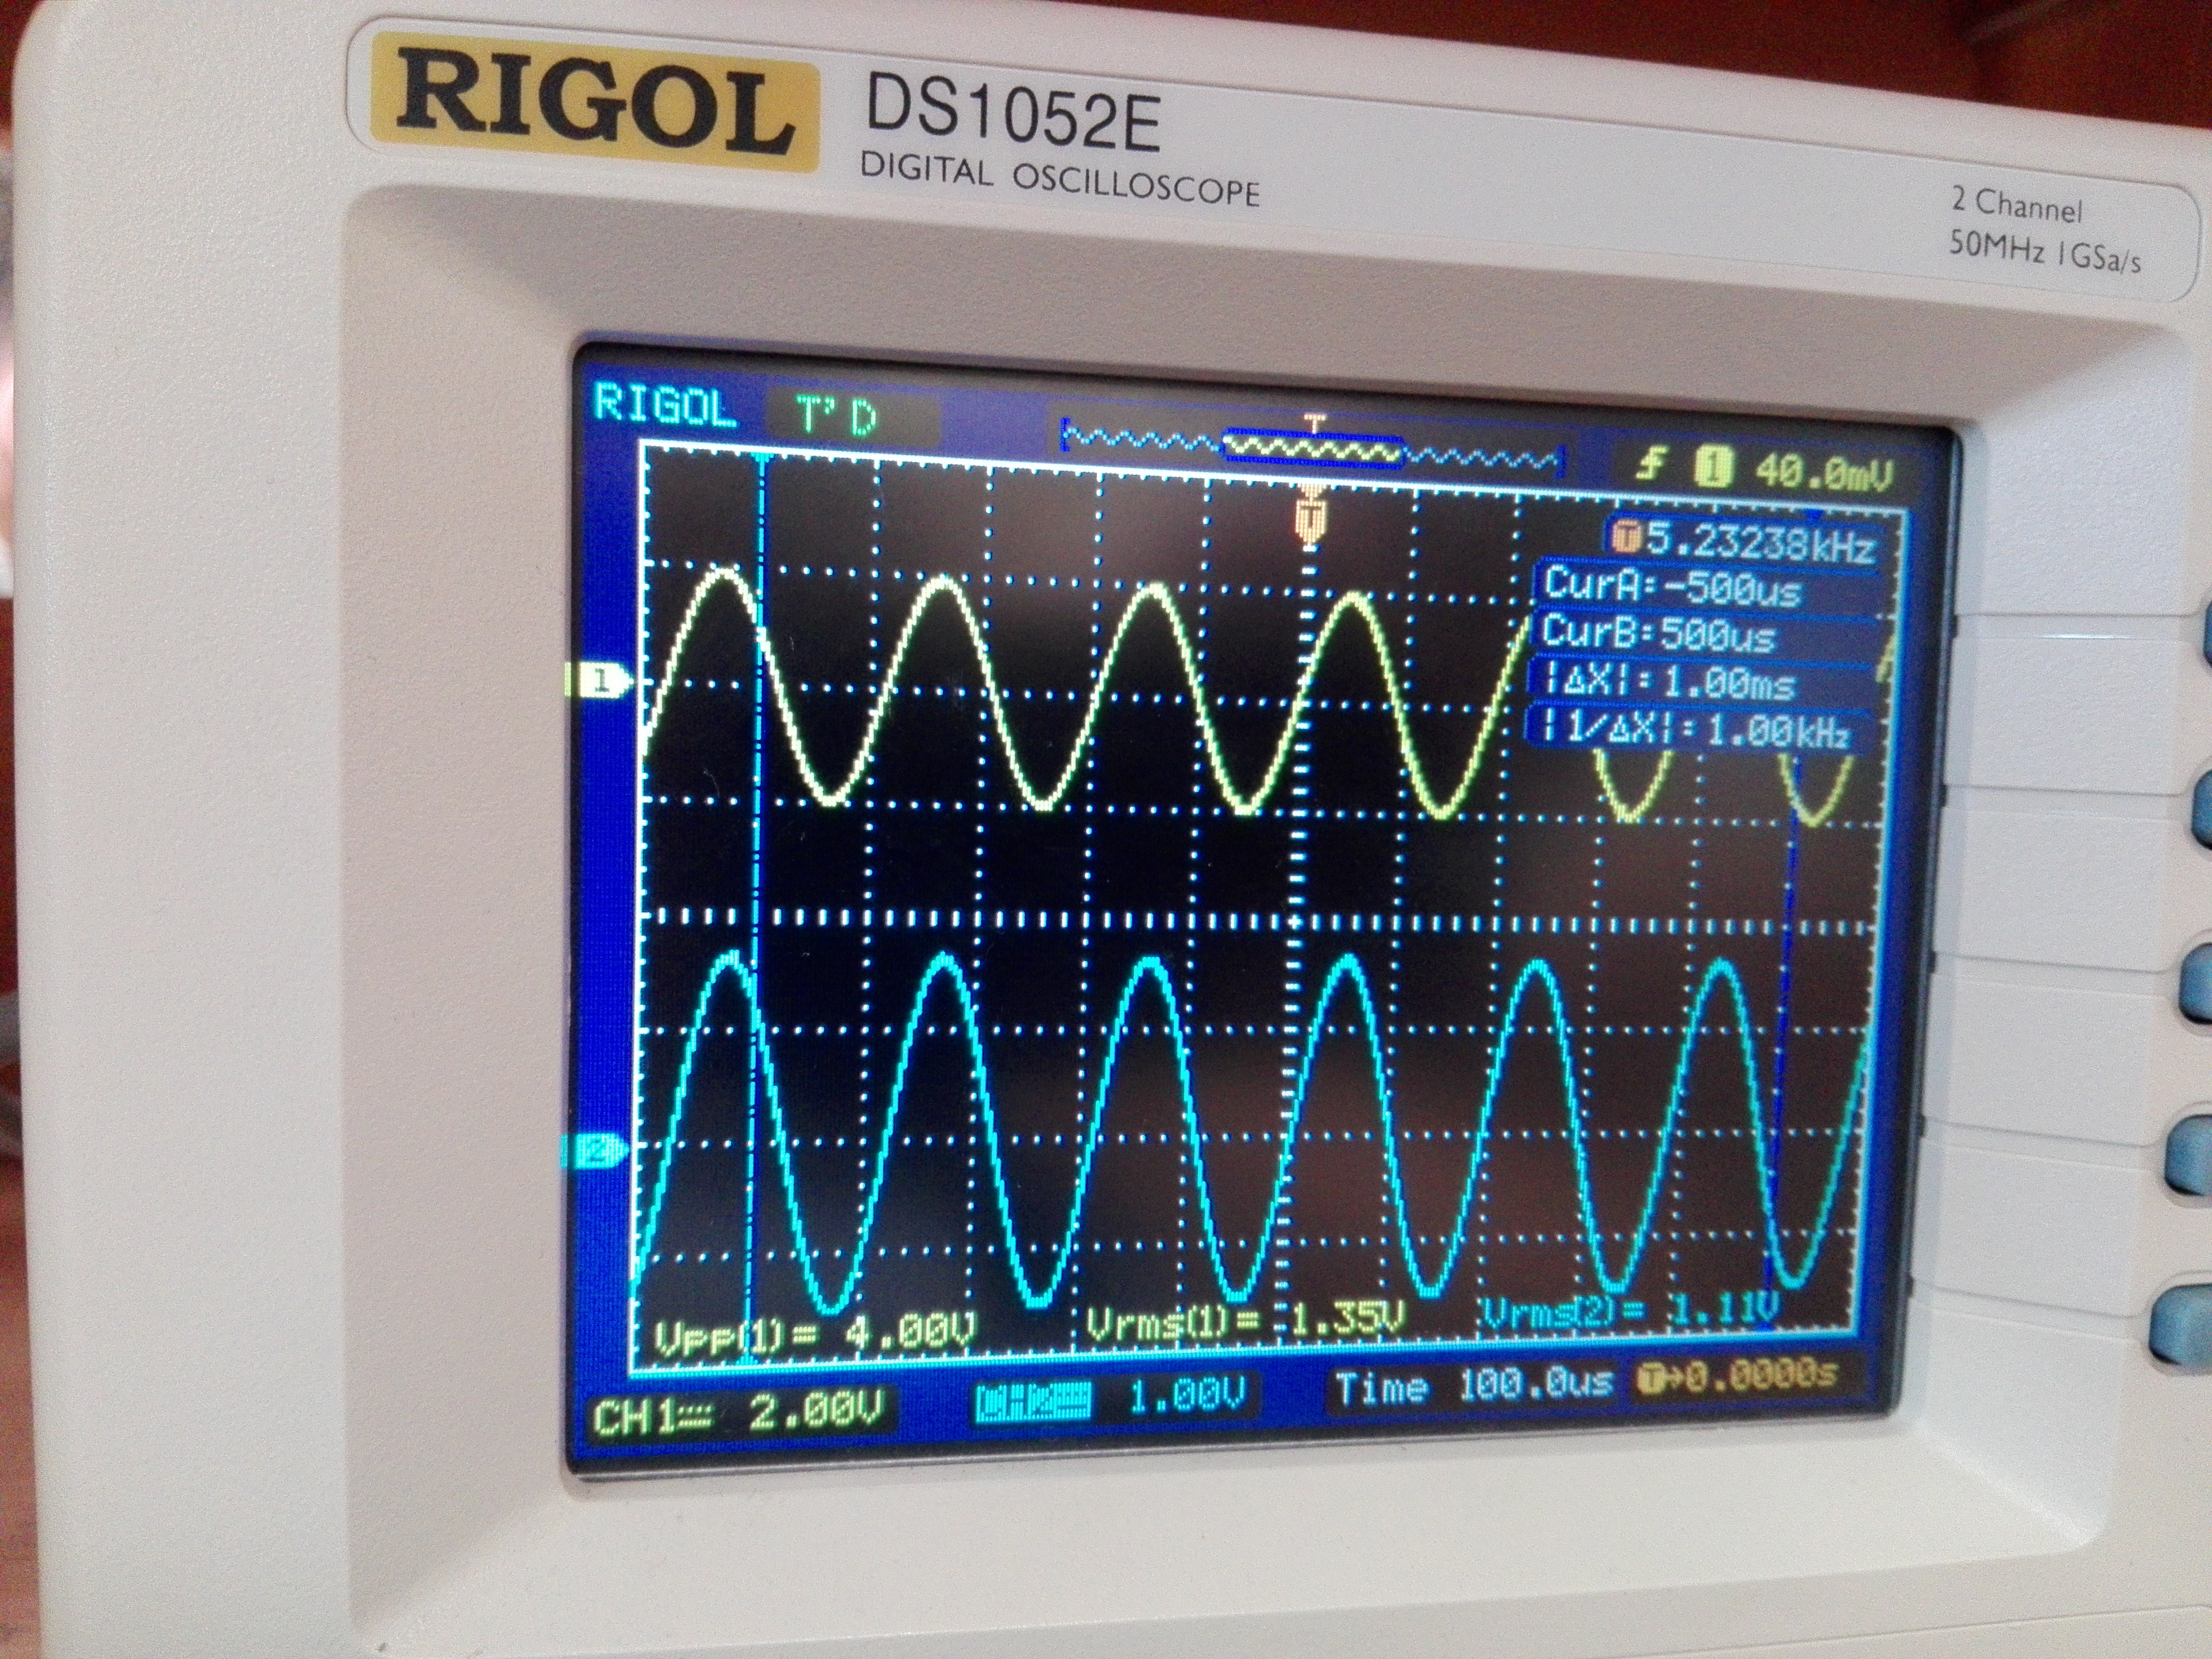
\includegraphics[width=\textwidth]{rezonans}

\section{Zadanie 9.}
Odczyt z ekranu oscyloskopu dla obwodu pobudzonego częstotliwością powyżej rezonansowej:\\
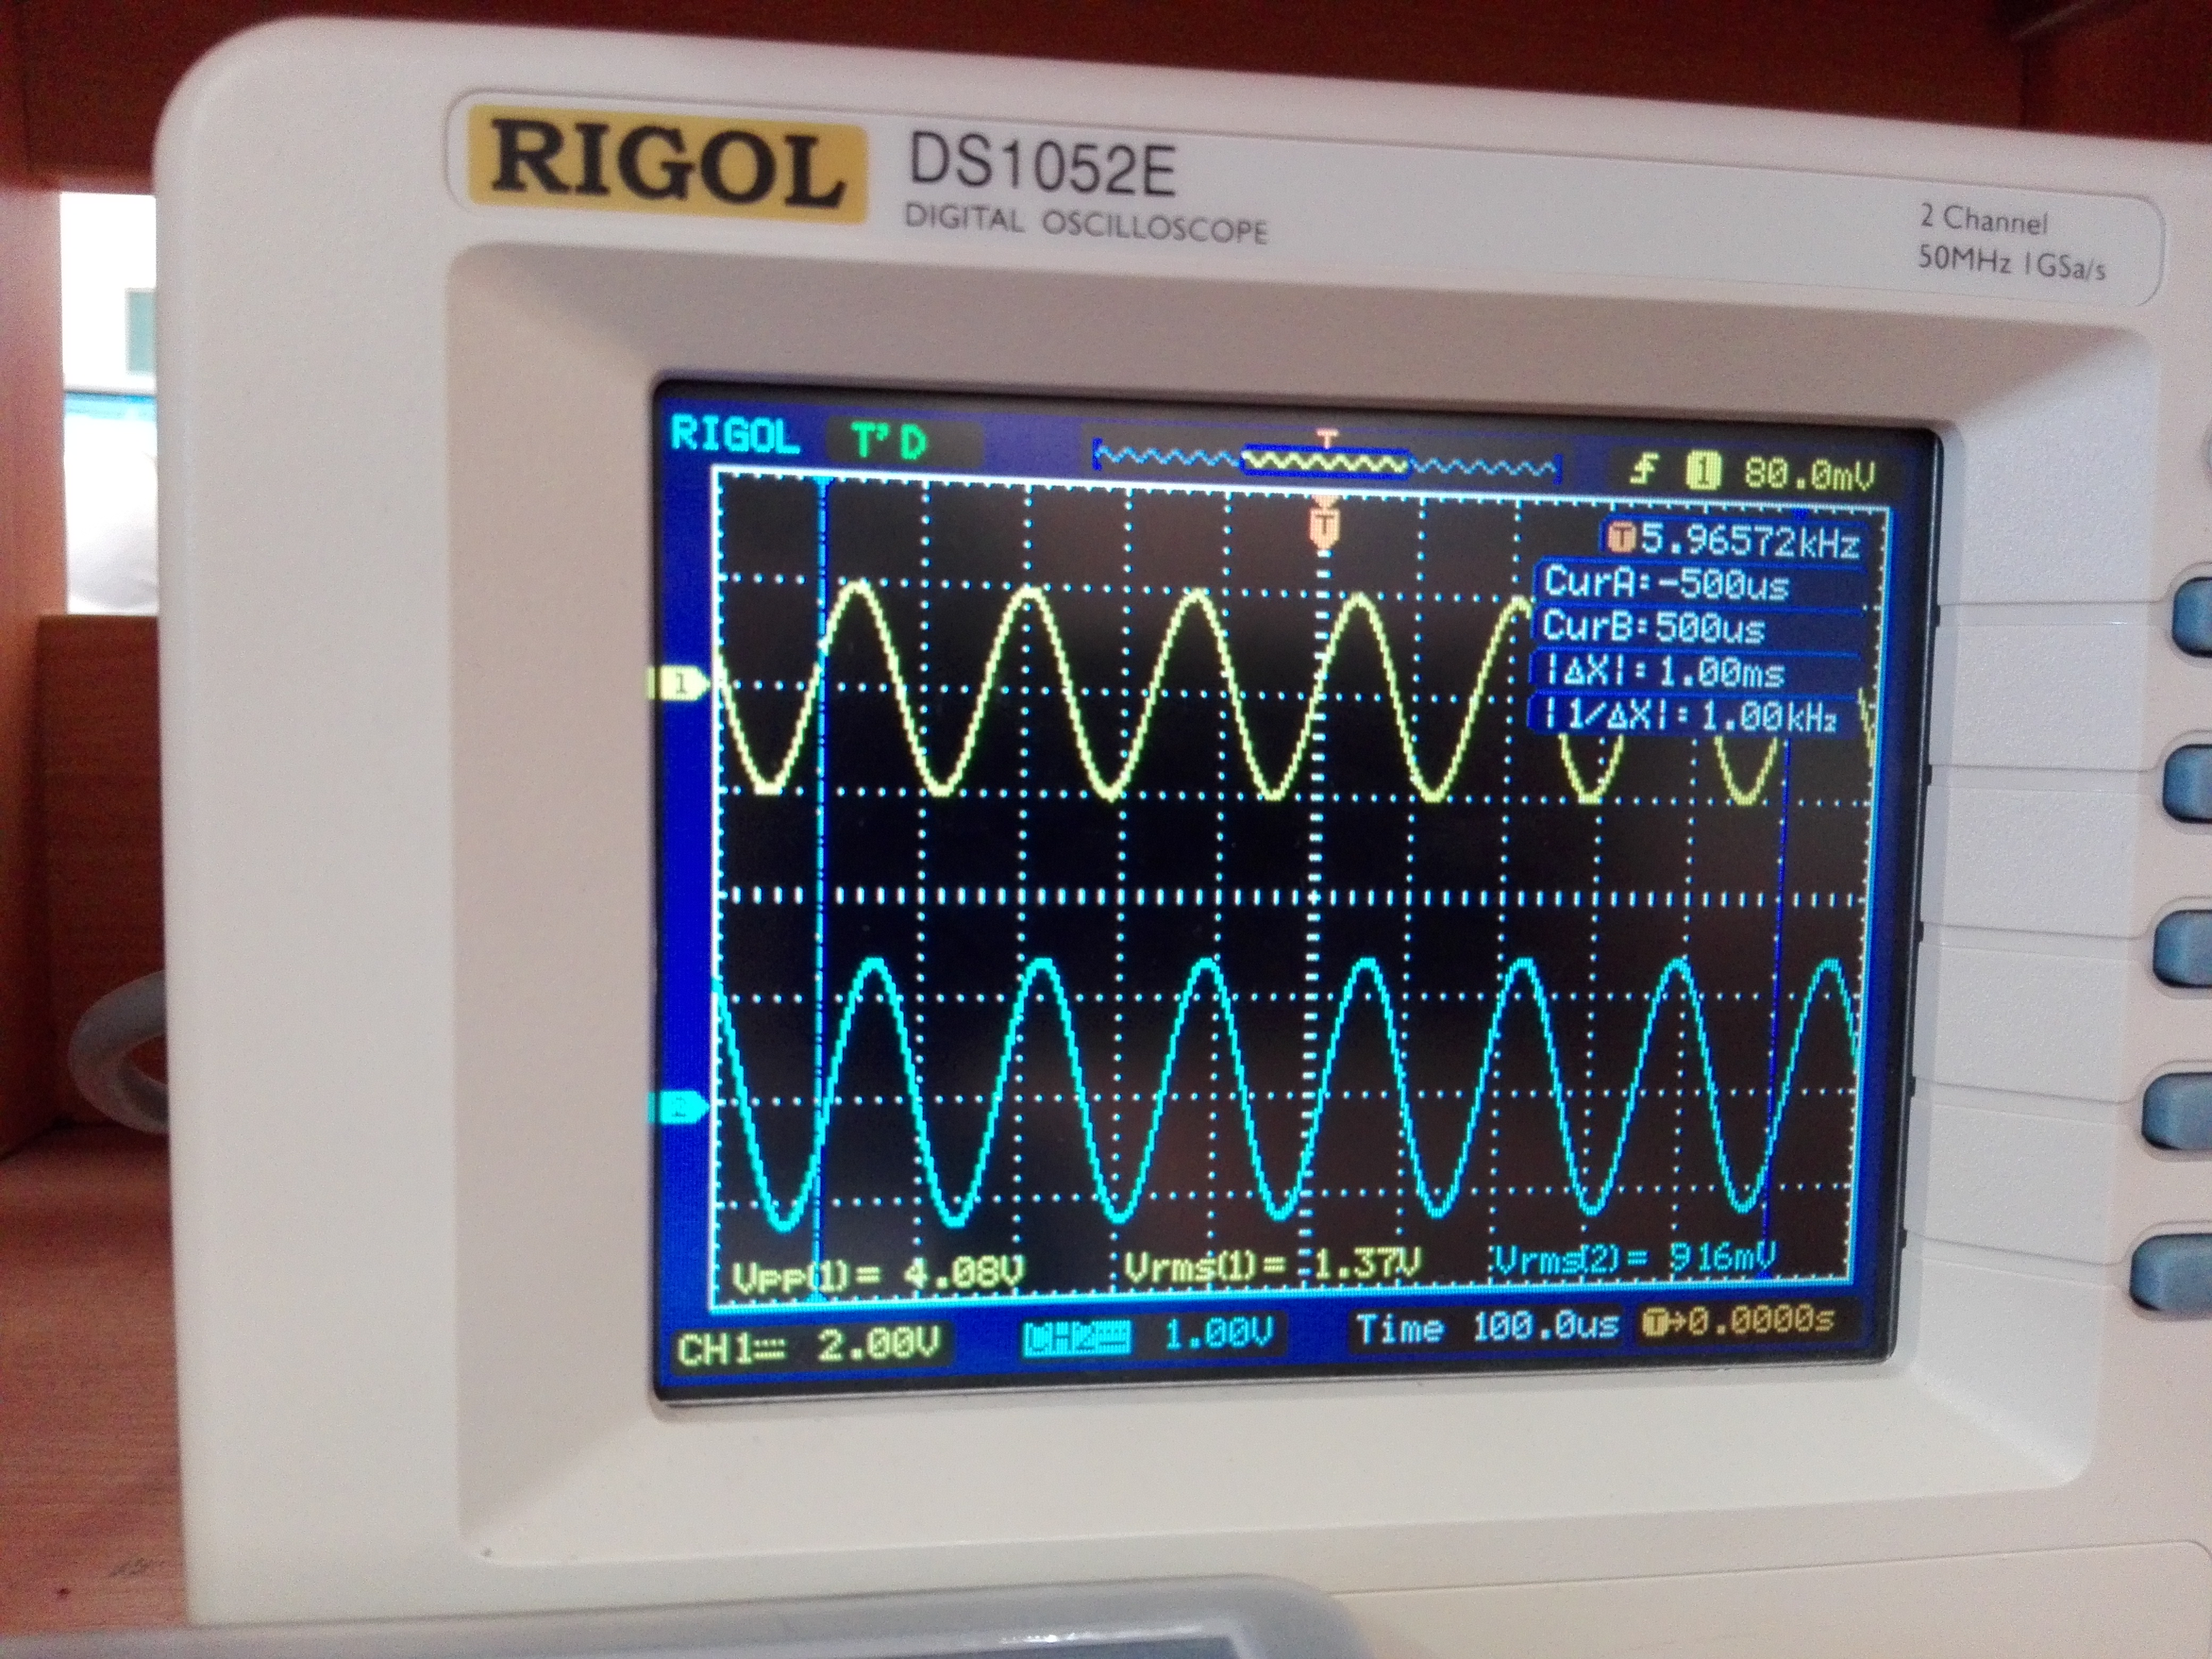
\includegraphics[width=\textwidth]{powyzej}
\newpage
Odczyt z ekranu oscyloskopu dla obwodu pobudzonego częstotliwością poniżej rezonansowej:\\
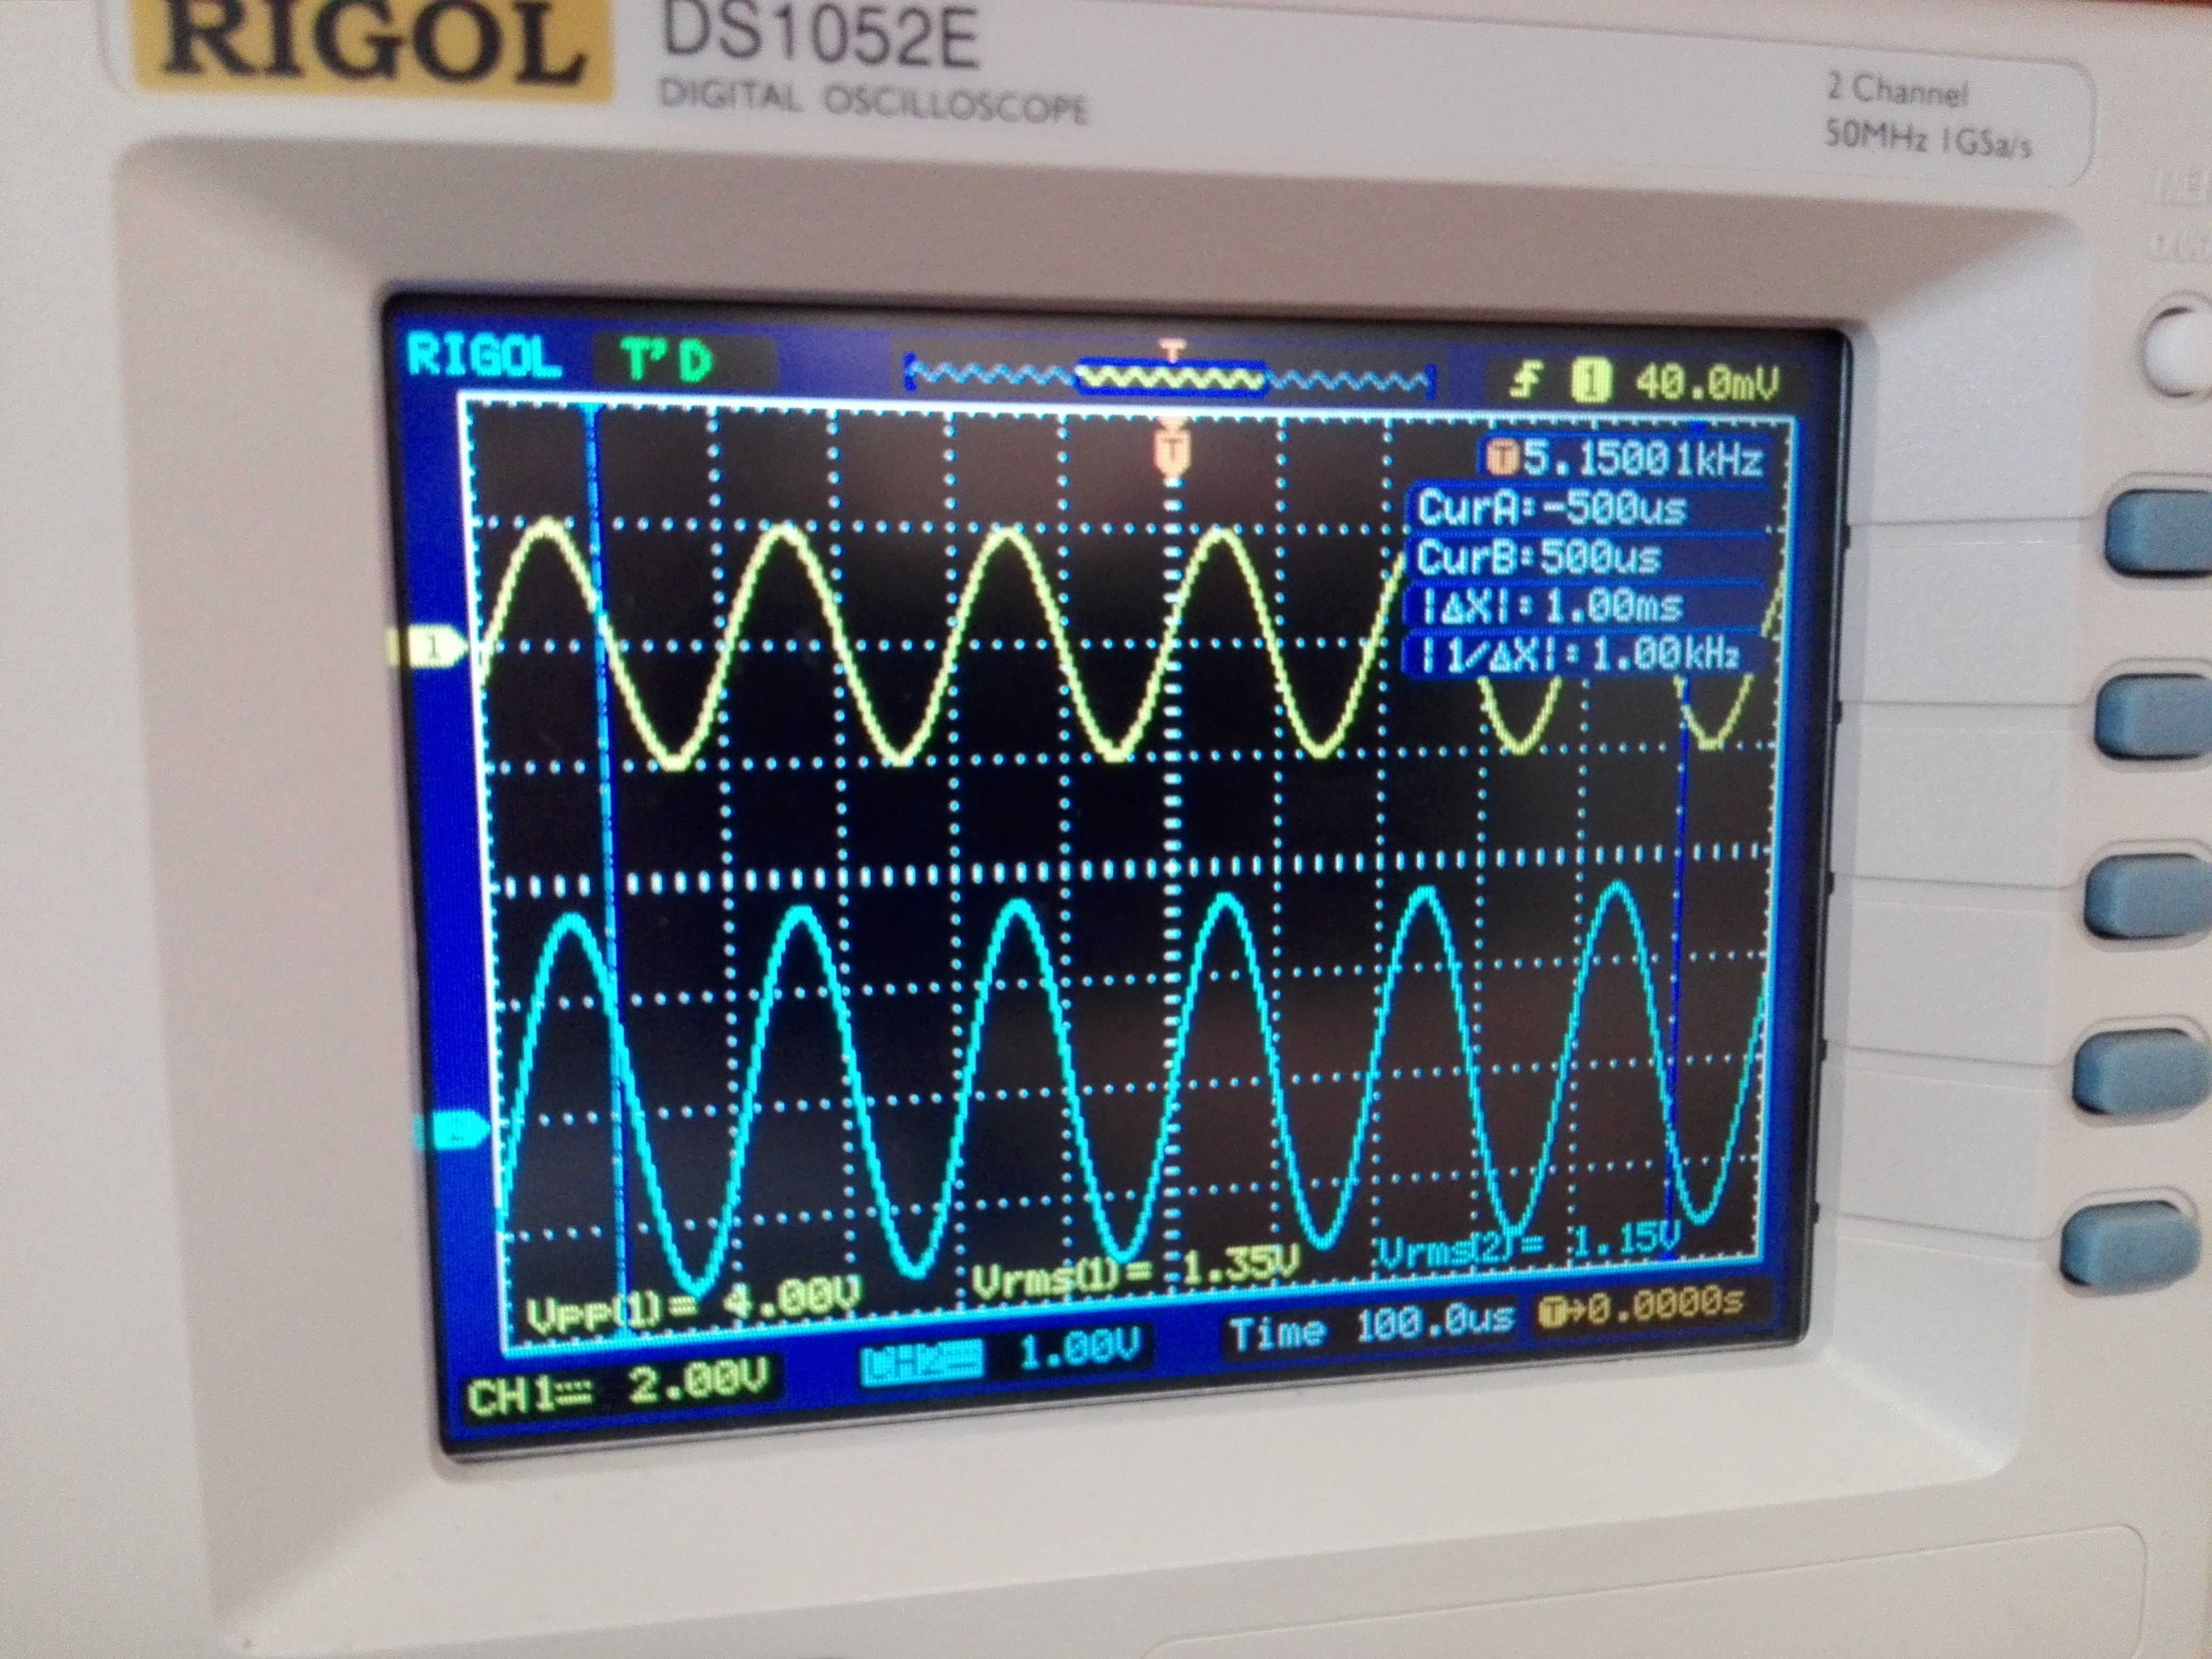
\includegraphics[width=\textwidth]{ponizej}

---COŚ O PRZESUNIĘCIACH FAZOWYCH---

\section{Zadanie 10.}
Wyznaczanie dobroci elementu indukcyjnego ze wzoru $Q_{L} = \frac{\omega_{0}L}{R_{L}}$ korzystając z wyznaczonych empirycznie parametrów.\\
$\omega_{0}=\frac{1}{\sqrt{LC}}$ - pulsacja rezonansowa obwodu
$$
Q_{L} = \frac{\frac{1}{\sqrt{69,78mH\cdot13,25nF}}\cdot69,78mH}{123,3\Omega} = 18,61
$$



\section{Wnioski}
------------------------------



\bibliography{IEEEabrv,refs}

\begin{thebibliography}{9}

\bibitem{rlc}
  W trakcie przeprowadzania doświadczeń i pisania sprawozdania zespół korzystał głównie z materiałów ze strony http://mariusznaumowicz.ddns.net/materialy.html oraz z wiedzy własnej.

\end{thebibliography}

\end{document}7